\documentclass{report}
\usepackage{graphicx} % Required for inserting images
\usepackage{subcaption}
\usepackage{booktabs} % For better table formatting
\usepackage{float}
\usepackage{hyperref} % Include the hyperref package for creating hyperlinks


\begin{document}
\begin{titlepage}
    \centerline{\Huge\textbf{IMPRESS Low Level Documentation}}
    
    \vspace*{1cm}
    
    \centerline{
\includegraphics[width=9cm]{hohenstein logo.jpg}}
    
    \vspace*{1.5cm}
    
    \centerline{\LARGE Bönnigheim, Germany}
    
    \vspace*{1cm}
    
    \centerline{\Large\textit{Illia Rohalskyi}}

    \vspace*{0.2cm}
    
    \centerline{\Large\textit{Dr. Igor Kogut}}

    \vspace*{0.2cm}
    
    \centerline{\Large\textit{Elias Brohammer}}
    
    \vspace*{1cm}
    
    \centerline{\Large\textit{Version 1: 11.12.2023}}
    
\end{titlepage}


\tableofcontents
\chapter{Introduction}
\section{Purpose of the Document}
The purpose of this document is to give a reader an overview of a project, it's structure and functionalities. It serves as a comprehensive yet concise document that could be read to understand the project scope, architecture and other essential details without delving into intricate technical details.

\section{Scope}
The scope of this document encompasses the entire "IMPRESS" project including its objectives, features, architecture, deployment strategy, and testing approach. The document does not delve into detailed technical implementation but provides an overview to help a reader understand the project's essence.

\section{Definitions}

\begin{description}
    \item[$\cdot$ \textbf{IMPRESS:}] The name of the project being documented.
    
    \item[$\cdot$ \textbf{System Architecture:}] The high-level structure and organization of the project's components and modules.
    
    \item[$\cdot$ \textbf{Use Cases:}] Scenarios that describe how users interact with the project and achieve their goals.
        
    \item[$\cdot$ \textbf{References:}] External resources and materials used as references during project planning and design.

    \item[$\cdot$ \textbf{Component:}] A modular and self-contained unit of the system that has specific functionalities. Components can interact with each other to achieve higher-level features.

    \item[$\cdot$ \textbf{Continuous Integration (CI):}] A software development practice that involves regularly integrating code changes into a shared repository. CI aims to detect and resolve integration issues early in the development cycle.

    \item[$\cdot$ \textbf{Continuous Deployment (CD):}] A software development practice where changes to code are automatically built, tested, and deployed to production environments. CD aims to reduce manual intervention, minimize deployment delays, and ensure that new features and bug fixes are quickly delivered to end-users.

    \item[$\cdot$ \textbf{Maintainability:}] The measure of how easily a software system can be modified, updated, extended, or repaired over its lifecycle. A maintainable system is designed with clear and organized code, well-documented components, and modular architecture, making it more cost-effective and efficient to manage and evolve.

\end{description}



\chapter{General Description}
\section{Product Perspective}
The project's primary focus is to develop a predictive model for surface tension and concentration of specific surfactants. Predicting surface tension holds significant importance due to its essential role in the textile manufacturing and textile service industry. Surface tension affects various processes like dyeing, finishing, printing, washing, rinsing and coating, which are integral to delivering high-quality fabrics and materials. Accurate predictions can lead to improved product outcomes, reduced costs, and enhanced overall efficiency in the textile services.

\section{Tools Used}

In our project, we rely on a variety of tools to effectively manage and enhance our work. These tools play a crucial role in enabling collaboration, version control, automation, and efficient project management.

\begin{itemize}
    \item[$\cdot$] \textbf{MLFlow:} MLFlow assists us in managing our machine learning models. It enables us to track different model versions, monitor their performance, and store associated artifacts. This allows us to make informed decisions when choosing which model to deploy.
    
    \item[$\cdot$] \textbf{DagsHub:} DagsHub serves as our collaborative platform for machine learning projects. It aids in version control, data sharing, and team collaboration. DagsHub ensures that our project components are well-organized and accessible to all team members.
    
    \item[$\cdot$] \textbf{DVC (Data Version Control):} DVC helps us manage and track changes to our datasets. It ensures that our data remains consistent and well-documented, making it easier to maintain reliable and accurate machine learning models.
    
    \item[$\cdot$] \textbf{Git/Github:} Git and GitHub are essential for version control and code collaboration. Git tracks changes to our codebase, while GitHub provides a platform for storing, sharing, and collaborating on code repositories.
    
    \item[$\cdot$] \textbf{Prefect:} Prefect is our tool for workflow automation. It allows us to define, schedule, and monitor complex workflows. Prefect improves efficiency by automating repetitive tasks and ensuring orderly execution.

    \item[$\cdot$] \textbf{GitHub Actions:} GitHub Actions automates tasks and workflows within GitHub repositories. It helps us maintain code quality by automating testing and deployment processes, reducing errors and ensuring a consistent codebase.

    \item[$\cdot$] \textbf{AWS:} AWS (Amazon Web Services) provides cloud infrastructure and services that support various aspects of our project, including computing resources, storage, and more.

    \item[$\cdot$] \textbf{Docker:} Docker is used for containerization, allowing us to package our applications and their dependencies into isolated containers for consistent deployment.

    \item[$\cdot$] \textbf{PostgreSQL:} PostgreSQL is our relational database management system. It stores and manages data crucial for our project's functionality.

    \item[$\cdot$] \textbf{Evidently:} Evidently is a Python library we use for monitoring and visualizing machine learning model performance, ensuring transparency and reliability in our models.
\end{itemize}

\section{General Constraints}
\subsection{General Constraints for MLOps Project}

\begin{itemize}
    \item[$\cdot$] Implement robust error handling and exception management to prevent application crashes. Provide meaningful error messages for troubleshooting.
    \item[$\cdot$] Maintain version control for trained models to track changes and revert to previous versions if necessary.
    \item[$\cdot$] Implement data versioning to ensure consistency across different stages of the pipeline.
\end{itemize}

\subsection{Object-Oriented Design Practices}

\begin{itemize}
    \item[$\cdot$] Utilize proper class and module organization to promote modularity and code reusability.
\end{itemize}

\subsection{Continuous Integration and Deployment (CI/CD)}

\begin{itemize}
    \item[$\cdot$] Set up an automated CI/CD pipeline to streamline the process of testing, building, and deploying code and models.
    \item[$\cdot$] Use tools for automating testing and deployment tasks.
    \item[$\cdot$] Employ versioned Docker containers to ensure consistent environments across different stages of the pipeline.
\end{itemize}

\subsection{Model Monitoring and Governance}

\begin{itemize}
    \item[$\cdot$] Continuously monitor the performance of deployed models using monitoring tools. Detect anomalies, concept drift, and degradation in model performance, triggering alerts.
    \item[$\cdot$] Implement model explainability techniques to provide insights into model predictions and decisions.
    \item[$\cdot$] Maintain a model registry to keep track of deployed models, their versions, and associated metadata.
    \item[$\cdot$] Establish a clear process for model retraining.
\end{itemize}

\section{Assumptions}

\begin{itemize}
    \item[$\cdot$] \textbf{Data Availability}: We assume that the required input data will be available in the expected format and structure. Any changes or variations in data schema may require adjustments in the data preprocessing and modeling stages.
    \item[$\cdot$] \textbf{Representative Training Data}: We assume that the training data used for model development accurately represents real-world scenarios. Any biases or limitations in the training data might affect the model's generalization and predictions.
    \item[$\cdot$] \textbf{Limited Scope of Features}: We assume that the features used for model training and prediction are relevant and encompass the most important aspects of the problem. Features not considered might impact the model's performance.
    \item[$\cdot$] \textbf{Monitoring and Maintenance}: We assume that regular monitoring and maintenance of the deployed models will be conducted to ensure their continued effectiveness. Any neglect in monitoring might lead to model degradation.
    \item[$\cdot$] \textbf{Resource Availability}: We assume that the required computational resources, such as memory, processing power, and storage, will be available for model training, deployment, and monitoring.
\end{itemize}



\chapter{System Architecture}
\section{Overall Architecture}

The architecture of the system is organized to provide a clear structure for both development and deployment. It consists of several key components and directories that contribute to the project's functionality. In this documentation, we have omitted unnecessary files and folders to provide a concise and focused representation of the system architecture, allowing for a clearer understanding of the key components and their relationships.
Now, let's provide an overview of the project structure with the assistance of a diagram:

\begin{figure}[h]
\centering
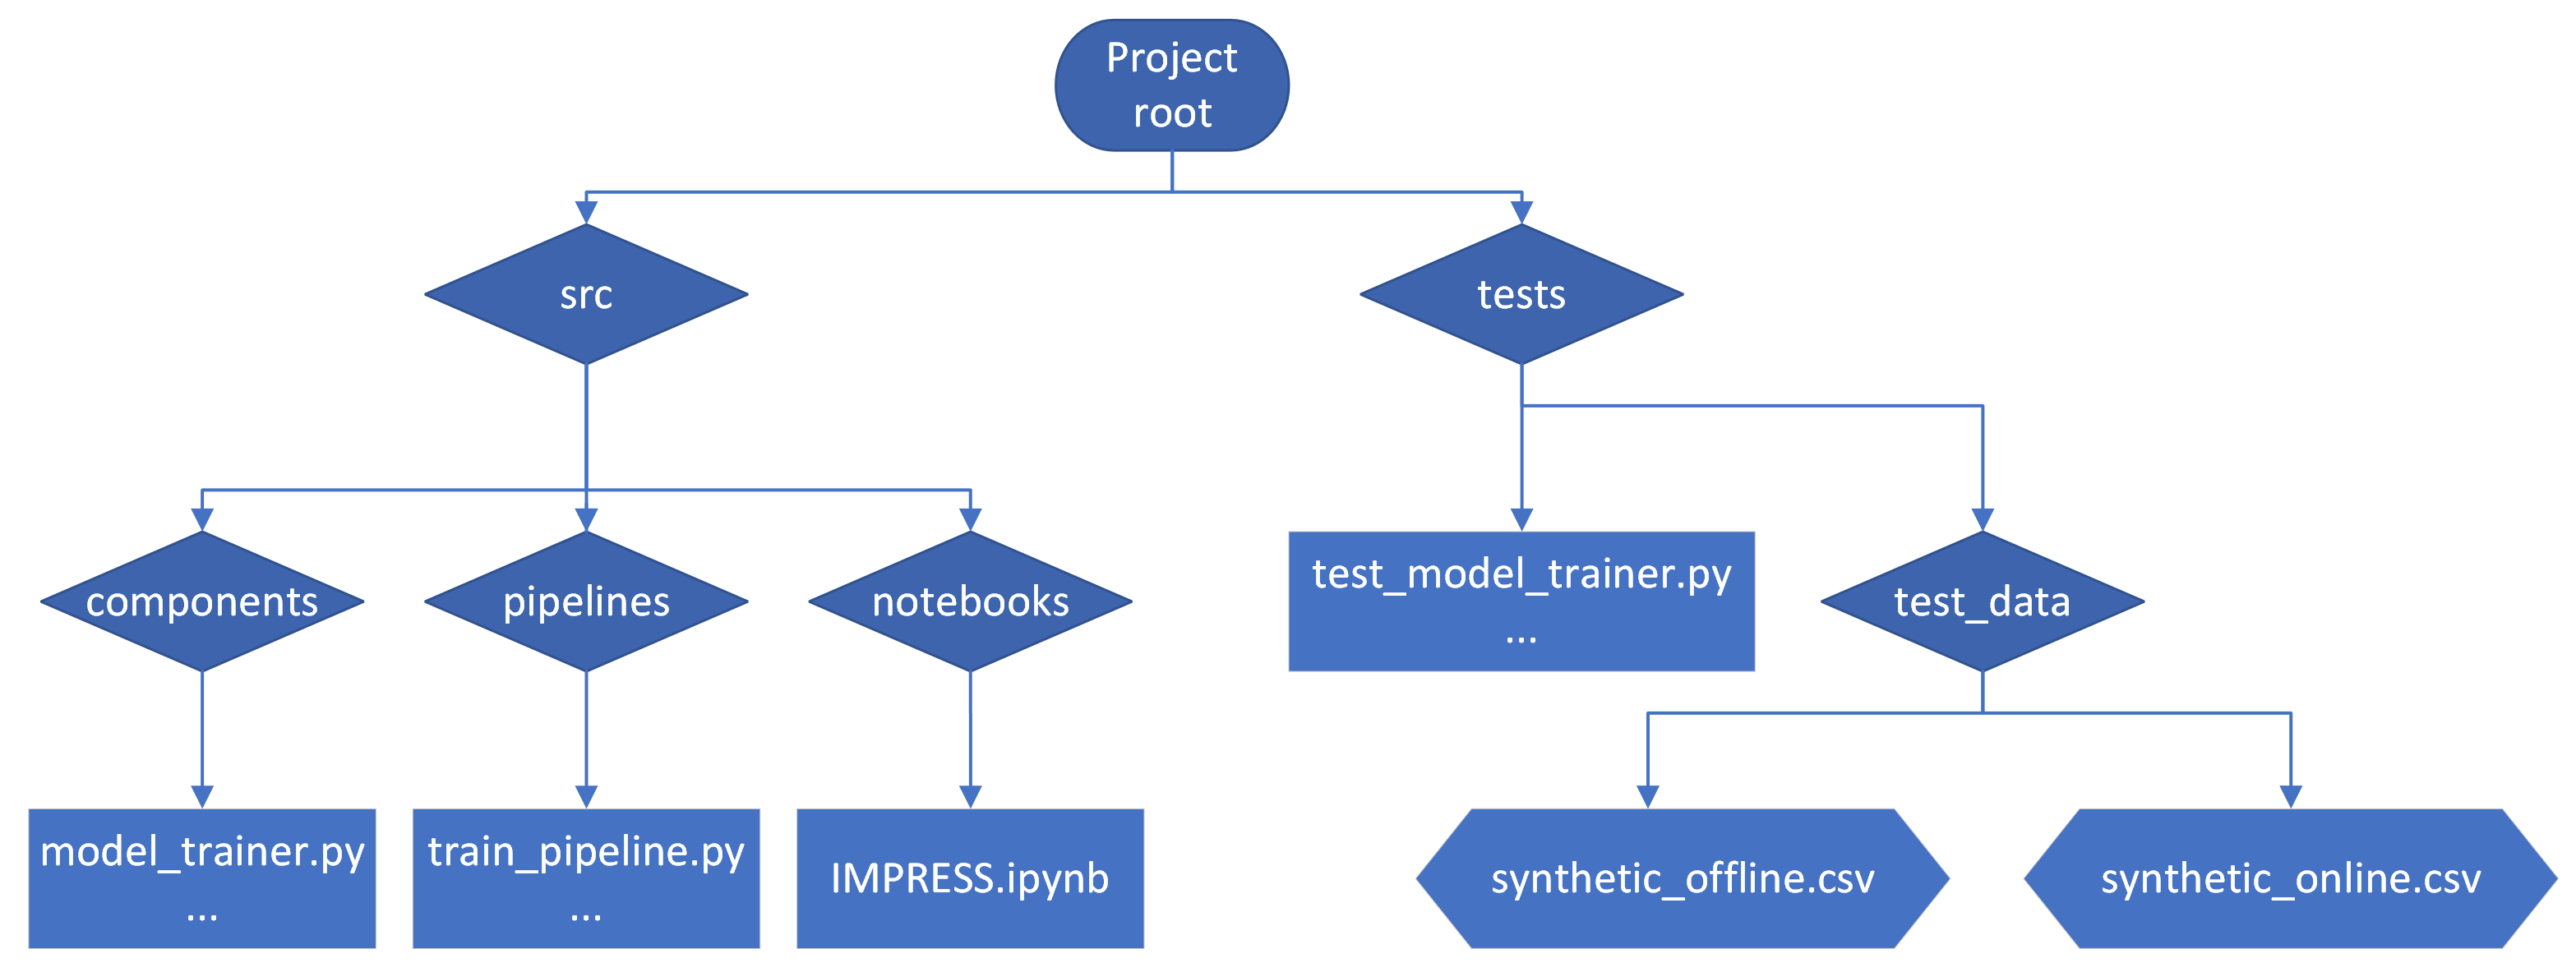
\includegraphics[width=\textwidth]{System_architecture.png}
\caption{Project Structure Diagram}
\label{fig:system-architecture}
\end{figure}

In the diagram above, you'll gain a visual understanding of how the project was structured. As we delve into details, this diagram will serve as a good reference point.
\subsection{Components (\texttt{src/components})}

This directory houses modular components that serve specific functions. These components can either be used independently or combined to accomplish more extensive tasks.

\subsection{Pipelines (\texttt{src/pipelines})}

The \texttt{pipelines} directory contains modules that orchestrate the execution of various components to achieve specific tasks. These pipelines are designed to streamline complex workflows, such as data transformation and model prediction.

\subsection{Testing (\texttt{tests})}

The \texttt{tests} directory is dedicated to testing the system's components and their integration. It includes unit tests for individual components as well as tests for the entire pipeline to ensure robust functionality.

\subsection{Notebooks (\texttt{src/notebooks})}

This directory contains Jupyter notebooks used for data analysis and exploration. While not directly involved in the project's core functionality, these notebooks are valuable for gaining insights and conducting experiments.

The architecture is designed to promote simplicity, modularity and maintainability. Components and pipelines can be developed and tested independently, making it easier to extend and enhance the system's capabilities. Additionally, the clear separation of concerns between components and the web application simplifies the development and deployment process.
\chapter{Model Training}
\section{Introduction}

In this chapter, we delve into the details of the model training process. Model training is a crucial step in our machine learning pipeline, where we build, fine-tune, and optimize machine learning models to make accurate predictions based on our dataset. This chapter provides an overview of the methodologies, tools, and techniques employed to create predictive models.

We begin this chapter by discussing the dataset and its preprocessing. Clean, well-structured data is the foundation of successful model training. Next, we explore the choice of algorithms and techniques suitable for our problem domain. We'll cover the training process, hyperparameter tuning, and evaluation metrics, ensuring our models perform optimally.

Throughout this chapter, we'll illustrate the practical aspects of model training with best practices. Whether you're new to machine learning or a seasoned data scientist, this chapter will provide valuable insights into our approach to building robust predictive models from softsensor data.

Let's dive into the fascinating world of model training and discover how it empowers our data-driven solutions.

\section{Exploratory Data Analysis (EDA)}

In this section, we conducted an Exploratory Data Analysis to understand the characteristics of the sensor data. We initially visualized the sensor time series, revealing significant variations among different sensors. Notably, each sensor exhibited distinct patterns, with some displaying considerable noise, while others showed more stable trends.

\subsection{Sensor Time Series Plots}

We present two representative sensor time series plots to illustrate the observed variations:

\begin{figure}[htbp]
    \begin{subfigure}{0.45\textwidth}
        \centering
        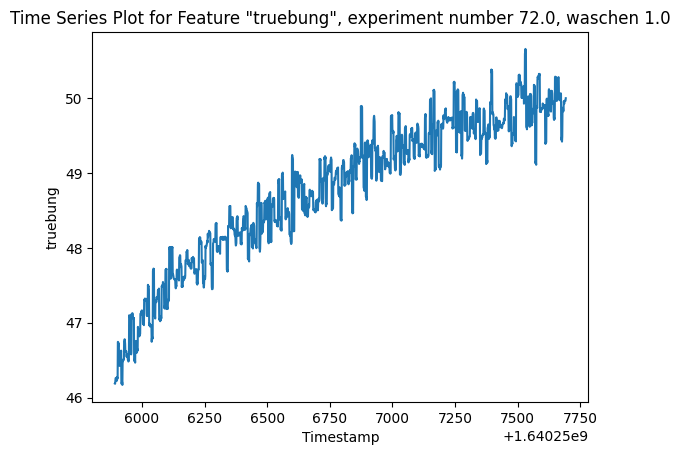
\includegraphics[width=\linewidth]{sensor_noisy_plot.png}
        \caption{Sensor with High Noise and Constant Increase}
        \label{fig:sensor_noisy}
    \end{subfigure}
    \hfill
    \begin{subfigure}{0.45\textwidth}
        \centering
        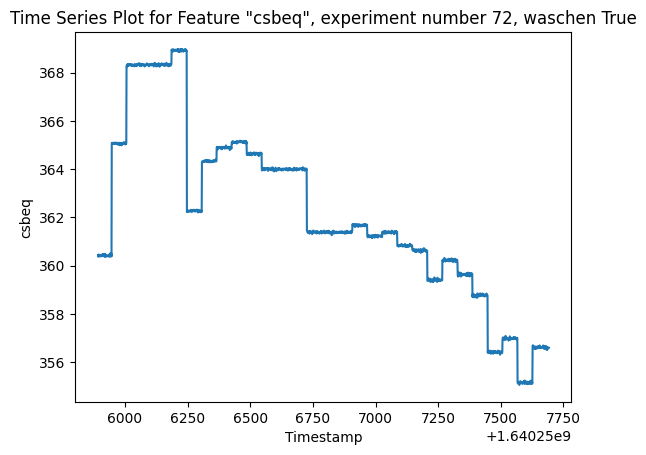
\includegraphics[width=\linewidth]{sensor_stable_plot.png}
        \caption{Sensor with Low Noise and Frequent Jumps}
        \label{fig:sensor_stable}
    \end{subfigure}
    \caption{Sensor Time Series Plots}
\end{figure}

As depicted in Figure \ref{fig:sensor_noisy}, Sensor 1 exhibits substantial noise and a constant upward trend, while Figure \ref{fig:sensor_stable} illustrates Sensor 2 with lower noise but frequent jumps in values.

\subsection{Correlation analysis}
Given the diverse nature of the sensor data, we decided to extract the mean from each sensor's time series. This aggregation aimed to capture the central tendency and simplify the subsequent analysis.

We computed the correlation matrix based on the mean values extracted from the sensors. Surprisingly, the correlation was low, suggesting a complex relationship among the features. The intricate nature of this relationship could potentially be captured by more sophisticated models, such as Random Forest or other tree-based models.

Below is the correlation matrix representing the relationships between different sensors:
\newpage
\begin{figure}
    \centering
    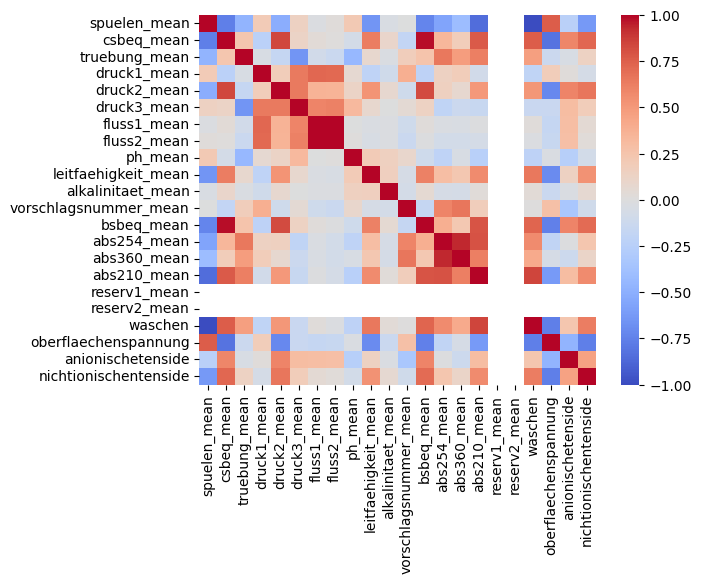
\includegraphics[width=1\textwidth]{correlation_matrix.png}
    \caption{Correlation Matrix of Sensor Data}
    \label{fig:correlation_matrix}
\end{figure}

This correlation matrix provides insights into the linear relationships between different sensors. However, the low correlation values indicate that more intricate patterns might exist.

Considering the complexity observed in the correlation analysis, further exploration with advanced machine learning models, such as Random Forest, could potentially unveil hidden relationships within the data.


\section{Feature Engineering}
Examining the correlation matrix in Figure \ref{fig:correlation_matrix}, a notable observation is the high correlation between surface tension and both anionic and nonionic surfactants. However, certain rows displayed NaN values, prompting the application of the MICE algorithm. MICE, an acronym for Multiple Imputation by Chained Equations, is an algorithm designed to predict missing data by leveraging the information from other available features. This method aims to fill in the gaps in the dataset, contributing to a more comprehensive and accurate analysis.
\begin{figure}[H]
    \begin{subfigure}[t]{0.48\textwidth}
        \centering
        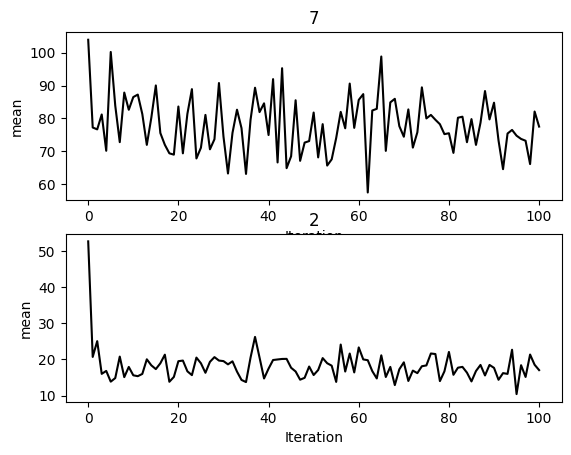
\includegraphics[width=\linewidth]{MICE_convergence.png}
        \caption{MICE Convergence: nonionic surfactants (top), anionic surfactants (bottom)}
        \label{fig:MICE_convergence}
    \end{subfigure}
    \hfill
    \begin{subfigure}[t]{0.48\textwidth}
        \centering
        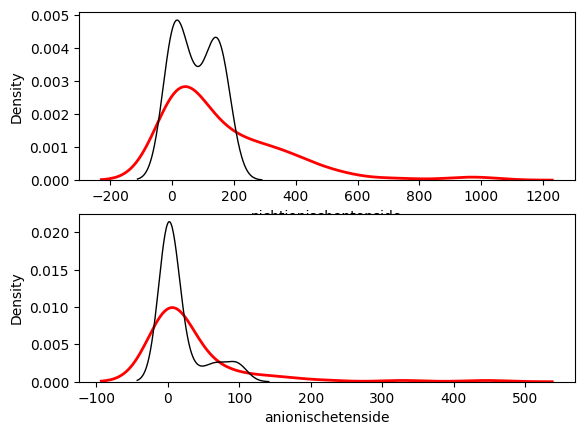
\includegraphics[width=\linewidth]{MICE_distributions.png}
        \caption{MICE Imputation Distribution: nonionic surfactants (top), anionic surfactants (bottom). Red line represents original data distribution, and the black line represents imputed data distribution}
        \label{fig:MICE_distribution}
    \end{subfigure}
    \caption{MICE Algorithm Results}
\end{figure}

Because the data was noisy, we considered using filter smoothing to reduce the noise in the time series. After attempting this approach, we found that it didn't provide significant benefits, so we decided to proceed without it. Below are the plots illustrating how the smoothing appeared:

\begin{figure}[h]
    \begin{subfigure}[t]{0.48\textwidth}
        \centering
        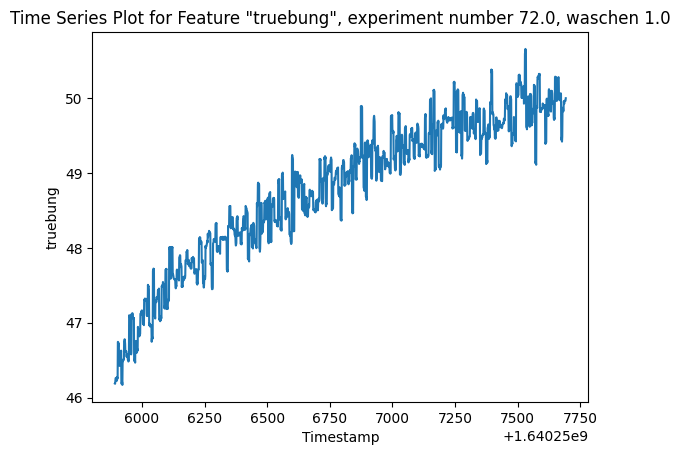
\includegraphics[width=\linewidth]{sensor_noisy_plot.png}
        \caption{Raw Signal}
        \label{fig:smoothing_a}
    \end{subfigure}
    \hfill
    \begin{subfigure}[t]{0.48\textwidth}
        \centering
        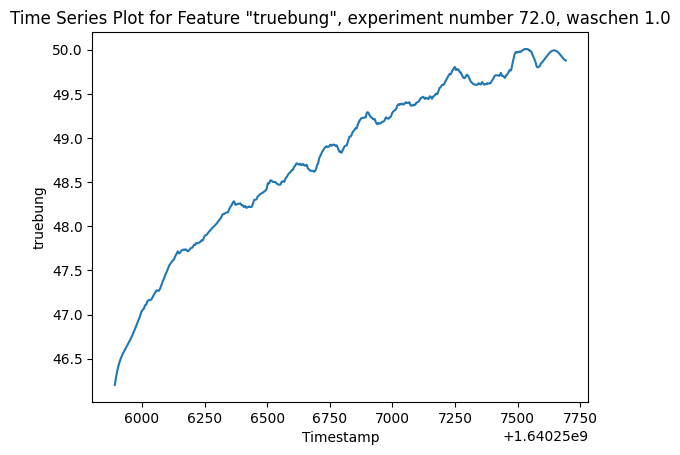
\includegraphics[width=\linewidth]{smoothing.png}
        \caption{Smoothed Signal}
        \label{fig:smoothing_b}
    \end{subfigure}
    \caption{Effect of Smoothing on Time Series}
\end{figure}

We employed a systematic approach to extract relevant information from our time series data. Our initial feature set consisted of mean, standard deviation, 25th percentile, median, and 75th percentile statistics from each time series feature. We believed that capturing these central tendencies and spread characteristics would provide valuable insights into the data.

Additionally, we experimented with augmenting these basic statistics by considering autocorrelation, trend statistics, and standard deviation differences. Although the latter seemed promising, it did not yield substantial improvements in our results.


To gain further insights into feature importance, we conducted feature importance plots, which highlighted that certain sensors had limited relevance for the model's performance.

\begin{figure}[H]
    \centering
    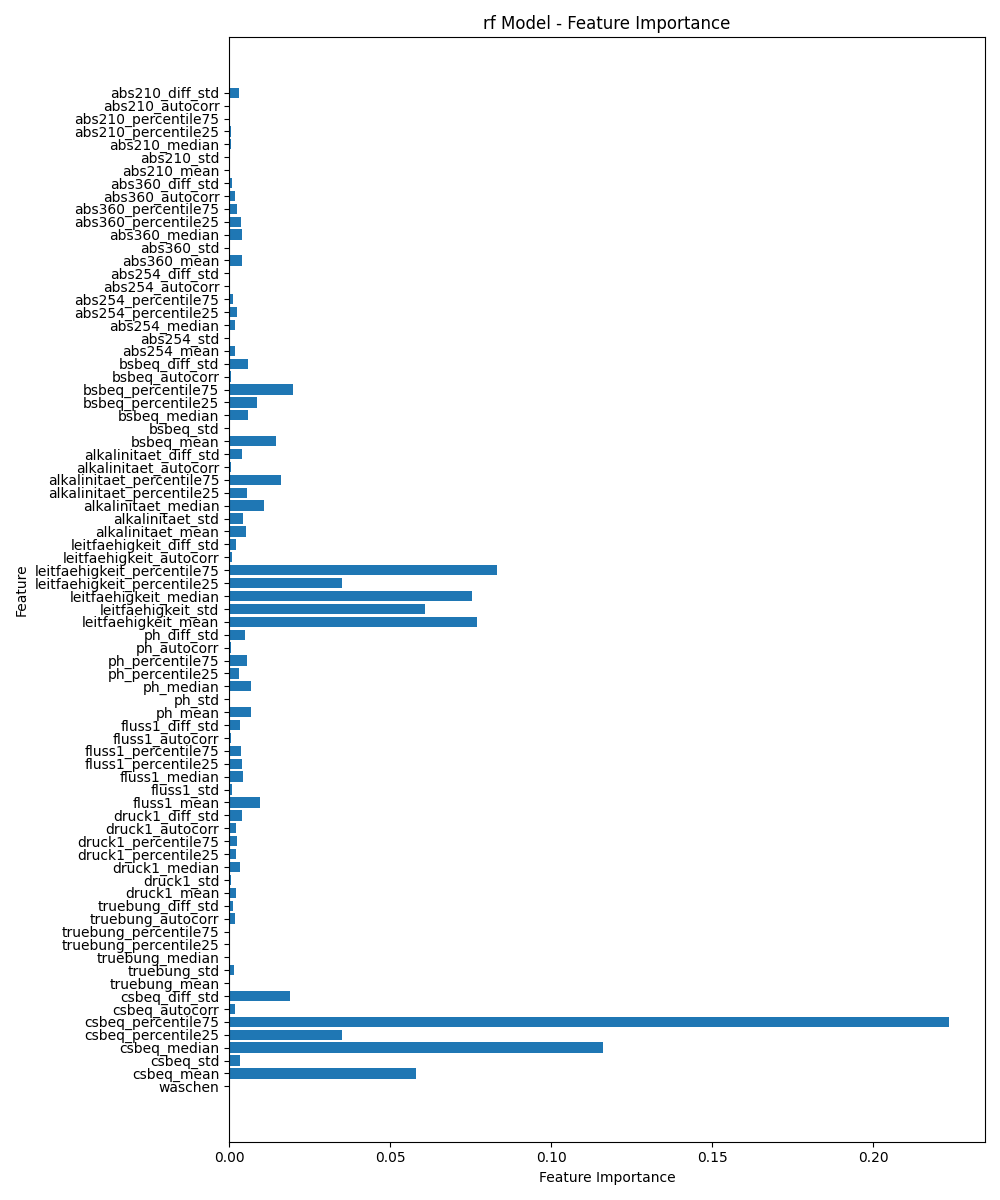
\includegraphics[width=1\textwidth]{feature_importance_plot.png}
    \caption{Feature Importance Plot for Random Forest}
    \label{fig:feature_importance_plot}
\end{figure}

In response, we conducted experiments using different subsets of sensors. First, we tested the model with only the most important sensors (conductivity, CODeq, turbidity), which resulted in similar performance to the full sensor set. Subsequently, we experimented with using only the least expensive sensors (turbidity, pressure, flow, pH, conductivity), which showed slightly worse results, with a mean absolute error (MAE) increase of less than 0,5. However, this approach significantly reduced costs. 

In comparison, initial experiment with all sensors (abs210, abs360, abs254, BODeq, CODeq, alkalinity, conductivity, pH, flow, pressure, turbidity) would cost us approximately 12,800 euros for sensors only. The experiment with most important sensors would lower it down to 8,800 euros. With the cheapest sensors approach, we would spend only 4,600 euros, which is almost three times less expensive then our initial experiment, and is almost twice less expensive then our most important sensors experiment. 

In the end, we decided to proceed with using the least expensive sensors, along with the essential statistical features we initially extracted: mean, standard deviation, 25th percentile, median, and 75th percentile. While we would have liked to explore more sophisticated modeling techniques, the limitation of available data prevented us from delving into deep learning or complex time series models.

This pragmatic approach allowed us to maintain good model performance with MAE score of 3.879 for surface tension while optimizing cost-effectiveness, aligning with our goal of leveraging machine learning for practical and efficient solutions.

\begin{table}[h]
    \centering
    \label{tab:ml_results}
    \begin{tabular}{lcccc}
        \toprule
        \textbf{Sensor Setup} & \textbf{ST MAE} & \textbf{NS MAE} & \textbf{AS MAE} & \textbf{Sensor Cost (\$)} \\
        \midrule
        All & 3.583 & \textbf{58.99} & \textbf{19.8} & 12,800 \\
        Most important & \textbf{3.558} & 67.2 & 20.82 & 8800 \\
        Cheapest & 3.879 & 64.36 & 23.38 & \textbf{4,600} \\
        \bottomrule
    \end{tabular}
    \caption{Machine Learning Results and Associated Costs for Various Sensor Setups. MAE: Mean Absolute Error. ST: Surface Tension, NS: Nonionic Surfactants, AS: Anionic Surfactants.}
\end{table}

\section{Training and Tuning}
In our training and tuning process, we adopted a well-thought-out strategy to ensure robust model performance. To begin with, we employed stratified cross-validation with 5 splits, while also reserving a separate test set for final model evaluation. The stratification was conducted across the washing and rinsing labels to guarantee an even representation of both in our validation sets. This approach aimed to mitigate any bias that could arise from imbalanced data distribution.

For hyperparameter tuning, we leveraged the TPEsampler with 100 optimization attempts. This method allowed us to explore a range of hyperparameters efficiently. We based our selection of hyperparameters on the average mean absolute error (MAE) across three scaled labels (surface tension, anionic surfactants, and nonionic surfactants) and five cross-validation splits. We employed two tree-based models for our experiments: the XGBoost Regressor and Random Forest. These models were chosen because the relationships within the data were complex and non-linear, making tree-based models well-suited to capture these nuances.

Ultimately, we decided to ensemble these two models using an averaging technique. We found that the Random Forest model exhibited slightly better accuracy and was assigned a weight of approximately 0.51 in the ensemble, while the XGBoost Regressor, although slightly less accurate, was still valuable and received a weight of around 0.49. This ensemble approach proved to be effective, as the combination of the two models demonstrated better generalization performance than either model individually.

Our approach to training and tuning focused on the practicality of implementing tree-based models, considering the complex and nonlinear nature of the relationships in the data. The ensemble technique further improved our model's overall performance, aligning with our goal of delivering practical and accurate solutions.

Throughout our training and tuning process, we logged all relevant metrics in MLflow, ensuring transparency and easy monitoring of model performance. Additionally, we registered our models, allowing for reproducibility and easy deployment in practical applications. This approach aligns with our goal of practicality and efficiency in the field of machine learning and MLOps.

\section{Retraining}
For the purpose of retraining the model, we've established a retraining pipeline. This pipeline allows you to specify the model's configuration using a data class within a script. By simply running this script, you can train the model with the predefined configuration. 

One of the significant advantages of this approach is its efficiency. Since the hyperparameters are already set in the configuration, there's no need for time-consuming hyperparameter tuning. This makes it an ideal choice when you need to quickly retrain the model or reproduce a specific experiment.

This retraining pipeline offers a practical and convenient solution for maintaining and updating your models, aligning with your goal of achieving quick and efficient results.

\chapter{Deployment}

Our deployment strategy is a critical component of our Machine Learning Operations (MLOps) process. In this chapter, we'll delve into our deployment pipeline and its two core sections, showcasing the tools and techniques we've employed to ensure seamless and efficient model deployment.

\section{AWS Deployment with Docker Containers}

When it comes to deploying our machine learning models, we've chosen Amazon Web Services (AWS) as our cloud service provider. AWS, being one of the largest and most renowned cloud service providers, offers the robust infrastructure and services needed for our deployment pipeline.

We've adopted a containerization approach using Docker to package our models and their dependencies. Our deployment pipeline consists of two Docker containers, each serving a specific purpose in the workflow. These containers are pushed to the Amazon Elastic Container Registry (ECR) as part of our automated deployment process.

To illustrate our deployment pipeline visually, please refer to the provided image showcasing the Continuous Integration/Continuous Deployment (CI/CD) setup. This visual aid outlines the sequence of events in our deployment process, from code changes to production-ready containers.

\begin{figure}[h]
\centering
\includegraphics[width=\textwidth]{Deployment_process.png}
\caption{Deployment Process Diagram}
\label{fig:system-architecture}
\end{figure}

Our CI/CD pipeline is powered by GitHub Actions, which orchestrates the entire deployment process. Inside GitHub Actions, we perform various tasks, including automated testing, linting to ensure code quality, and model retrieval from MLflow. Only models marked as "Production" are included in the deployment pipeline. Subsequently, we push two container images with different tags to a single ECR repository.

\section{Deployment Pipelines for Prediction and Monitoring}

In the context of our deployment strategy, we have two distinct deployment pipelines, each serving a unique function.

The first pipeline, known as the "Prediction Pipeline" is dedicated to generating predictions through the utilization of our machine learning models. Its primary function involves retrieving relevant data from the PostgreSQL database hosted on the AWS Relational Database Service (RDS). Once the data is acquired, the pipeline seamlessly executes our models, leveraging their analytical capabilities. Subsequently, the computed predictions are then deposited into a designated table within the same database. This pipeline ensures that our models are actively providing predictions for real-world data, enabling us to leverage the power of machine learning in practical applications.

\begin{figure}[H]
    \centering
    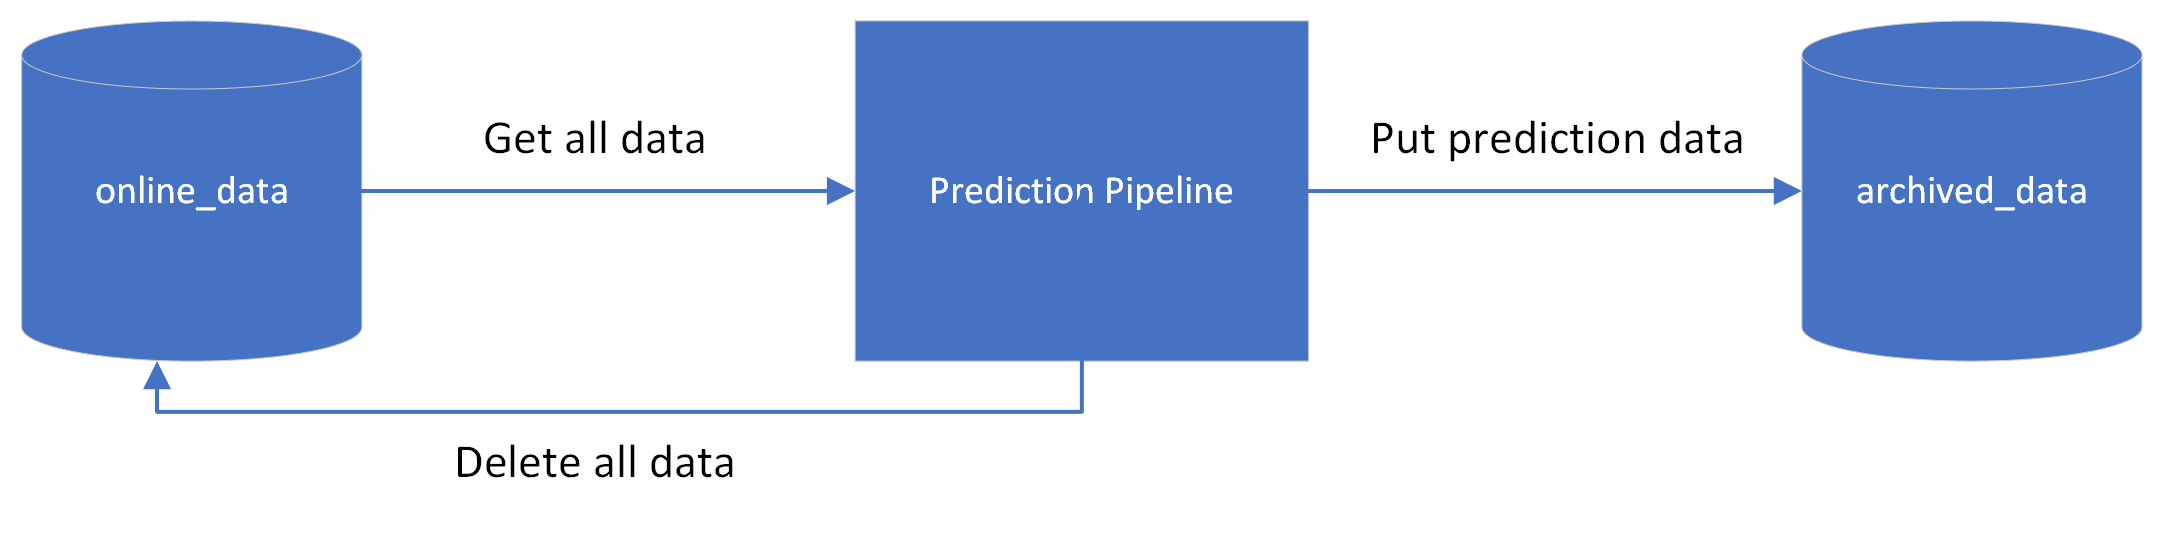
\includegraphics[width=0.8\linewidth]{prediction_pipeline.png}
    \caption{Prediction Pipeline and Database Tables Interactions}
    \label{fig:prediction_pipeline}
\end{figure}


The second pipeline, termed the "Monitoring Pipeline," plays a crucial role in data quality and drift monitoring. This pipeline relies on the table containing predictions and training data, that would be pulled from DVC, to monitor incoming data and identify potential drift or anomalies. When drift is detected, the monitoring pipeline generates clear and detailed reports. These reports are then sent via email to relevant stakeholders, allowing for prompt action and maintenance of model accuracy. It utilizes 90\% of the data, ensuring that the remaining 10\% remains unaltered in case it was recently predicted by the prediction pipeline and has not undergone inspection.

\begin{figure}[H]
    \centering
    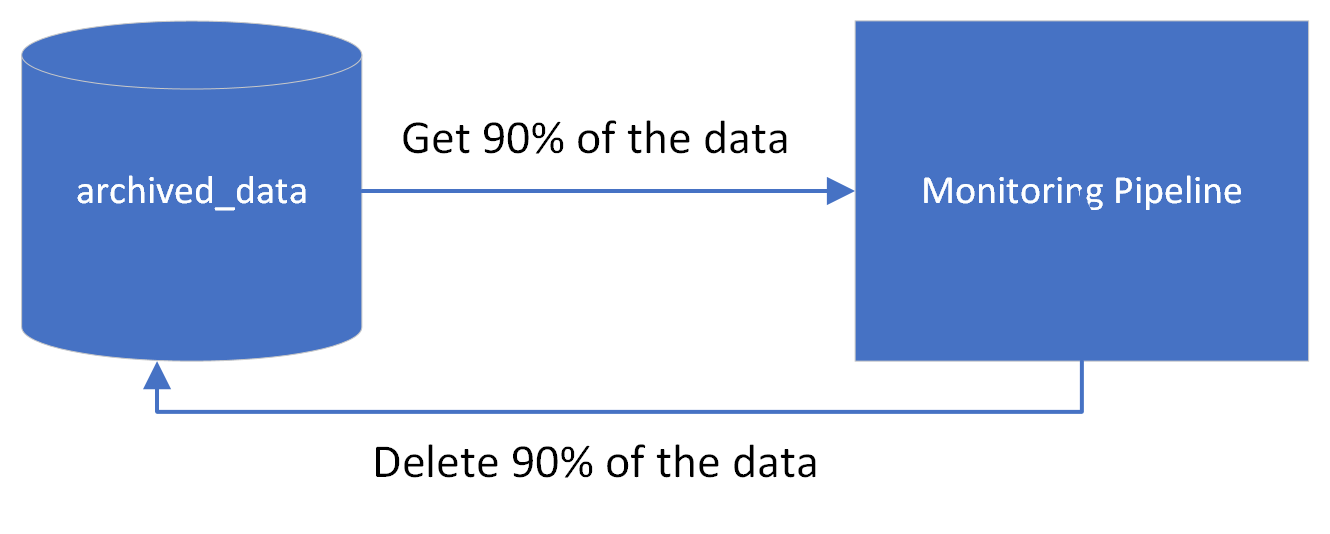
\includegraphics[width=0.7\linewidth]{monitoring_pipeline.png}
    \caption{Monitoring Pipeline and Database Tables Interactions}
    \label{fig:monitoring_pipeline}
\end{figure}

Our deployment strategy is designed for efficiency, reliability, and real-time adaptability, ensuring that our machine learning models are not only accurate but also robust in real-world scenarios. By dividing our deployment into these two dedicated pipelines, we can address both prediction and data quality monitoring, meeting our goal of providing practical and valuable solutions in the field of machine learning and MLOps.


\chapter{Testing Overview}

Testing is a fundamental aspect of ensuring the reliability and functionality of our machine learning models and deployment pipelines. In this chapter, we provide an overview of our testing strategies, encompassing both unit tests and integration tests. We also highlight the use of synthetic data and separate database tables for testing purposes.

\section{Unit Tests}

Unit tests are a crucial component of our testing strategy. They serve the purpose of verifying the correctness and functionality of individual components within our software ecosystem. Our unit tests are designed to check the behavior of specific functions, modules, or classes in isolation, ensuring that each piece of code operates as expected.

These unit tests are executed within our Continuous Integration/Continuous Deployment (CI/CD) pipeline, specifically in GitHub Actions. The results of these tests provide us with valuable feedback on the health of our software components. Any unexpected behavior or errors are promptly identified, allowing for rapid resolution.

To facilitate our unit testing process, we have created synthetic data sets that are used as inputs.

\section{Integration Tests}

In addition to unit tests, we conduct integration tests to evaluate the interactions and compatibility of our entire pipeline. Integration tests assess how different components work together as a whole and ensure that data flows smoothly from end to end.

Our integration tests are also orchestrated within GitHub Actions, providing a holistic assessment of the entire deployment process. These tests involve the utilization of synthetic data and separate tables within the Amazon Relational Database Service (RDS) created explicitly for testing purposes.

These dedicated testing tables enable us to simulate real-world scenarios and assess the robustness of our deployment pipeline. By running integration tests, we can identify any inconsistencies, bottlenecks, or issues in the flow of data and predictions, guaranteeing that our deployment remains reliable and stable.

Our approach to testing, which includes both unit tests and integration tests, plays a pivotal role in ensuring the functionality and reliability of our machine learning solution. The use of synthetic data and dedicated testing tables enhances our ability to capture and resolve issues, ultimately contributing to the quality and effectiveness of our software ecosystem.

\chapter{Possible Use Cases}
\section{Textile Industry}
The textile manufacturing industry and industrial laundering services utilize a high number of detergents for dyeing, washing, and rinsing processes. Often these processes are linked to inefficiency in resource management and failures in process quality. Particularly, the prediction of surface tension and concentration of surfactants can be used for automatization of the rinsing process in both industries. The sensor array that measures the time series will be integrated via bypass in the rinsing process. If some threshold values of surface tension, i.e. organic contaminants, are exceeded, the rinsing process may be prolonged or more water is added to the rinsing process. Thus, automatically is ensured that the fabrics are free of organic contaminants at the end of manufacturing/textile cleaning process. This ML application will lead do decrease in rewash rate, process failures, fabric replacement and subsequently save resources. The amortization time of such system is expected to be 1 to 3 years.
\section{Parts Cleaning Industry (Automotive Suppliers)}
Industrial parts cleaning is an important industrial branch that uses different solvent–surfactant mixtures to remove contaminants, like grease, from surface of metallic parts. In this way, subsequent processes like assembling of metallic parts can be realized without failures. Here so-called cleaning bathes are used, and the process water is circulated through filtration devices. To ensure the concentration of surfactant solution in the cleaning bath and subsequent rinsing processes, efficient sensor systems are necessary, which not exist in the moment. The cost-efficient sensor array could be easily installed in different cleaning steps and the ML application would derive data, predict surface tension and concentration of surfactants. Based on the monitoring, an efficient controlling algorithm could be set up. The novel technology would lead to faster and more cost-efficient process workflow, as well as ensure that minimum of resources are utilized for the processes.
\chapter{Retrospective}

\section{Project Achievements}
\begin{itemize}
  \item[$\cdot$] \textbf{Development of a Machine Learning Solution:} The project successfully delivered a machine learning solution that predicts surface tension using soft sensors, demonstrating the feasibility of this approach.
  
  \item[$\cdot$] \textbf{Integration with Cloud Technologies:} The solution effectively leveraged cloud technologies, particularly AWS, for data storage, deployment, and scalability, enhancing the project's efficiency and accessibility.
  
  \item[$\cdot$] \textbf{Unit and Integration Testing:} Comprehensive unit and integration tests were implemented in the CI/CD pipeline, ensuring the reliability and robustness of the entire system.
  
  \item[$\cdot$] \textbf{Use of Generic Project Framework:} Our project serves as a valuable reference for soft sensor machine learning. The framework we established can be adapted for similar projects in the future, providing a reusable and scalable solution.

  
  \item[$\cdot$] \textbf{Model Monitoring Implementation:}
    We successfully implemented a robust model monitoring system as part of the project. This system continuously tracks the performance of our machine learning models, providing insights into their reliability. Model monitoring is crucial for ensuring that our predictions remain accurate and reliable in dynamic real-world scenarios.

\end{itemize}

\section{Challenges Faced}
\begin{itemize}
  \item[$\cdot$] \textbf{Data Availability and Quality:} A significant challenge was encountered due to the limited and messy nature of the available data. This constraint hindered the development and testing phases of the project.
  
  \item[$\cdot$] \textbf{Time Constraints:} Time limitations affected the project's completeness and perfection. More time would have allowed for deeper exploration and optimization of various aspects.
  
  \item[$\cdot$] \textbf{Online Deployment Considerations:} While online deployment was considered to enable real-time data-driven predictions, it was deemed cost-inefficient and time-consuming, leading to the adoption of batch deployment.
\end{itemize}

\section{Areas for Improvement}
\begin{itemize}
  \item[$\cdot$] \textbf{Data Quality and Quantity:} Improving the quality and quantity of available data is essential to enhance model performance and reliability.
  
  \item[$\cdot$] \textbf{Project Timeline:} Extending the project timeline would allow for more thorough implementation, that could be more extensible. Config files could be created to make the project even more maintainable and flexible. Additionally, more metrics could be added, such as R-squared.
  
  \item[$\cdot$] \textbf{Online Deployment Implementation:} If resource availability permits, exploring and implementing online deployment for real-time predictions could be considered for more dynamic applications.
\end{itemize}


\end{document}
